% TODO: Explaination of the syntatic algorithm
% TODO: Perhaps some more (or more detailed) benchmarking 
\documentclass[a4paper,notitlepage]{scrartcl}

\usepackage{amsmath}
\usepackage{amssymb}
\usepackage{minted}
\usepackage[margin=2cm]{geometry}
\usepackage[final]{pdfpages}

% Use the nicer phi
\let\phi\varphi

\title{Conjunctive Normal Form}
\author{Bill Noble\\ Tim van der Molen}
\date{January 2014}

\begin{document}
\maketitle

Conjunctive normal form (CNF) is the standard notation for formulas in predicate
        and propositional logic.
A formula in CNF consists of a series of conjunctions containing subformulas
        which are only disjunctions of atomic propositions or their negations.
We use `and' and `or' as list operators.
Thus a formula whose main connective is `and' or `or' is a pair, the operator
        and a list of conjuncts or disjuncts.
For this reason, a formula in CNF contains (at most) one `and' operator.
Besides being standard notation, CNF is advantageous because it can speed up the
        evaluation of long formulas.
Disjunctive normal form (DNF) is the `or' analog to CNF. A formula in DNF is
        a single `or' list of subformulas made up of `and' lists of atomic
        formulas and their negations.

\section{The Syntactic Algorithm}
\begin{minted}[frame=single]{python}
# Helper function for cnf().
def cnf_do(f):
    if atom(f) or f[0] == 'not':
        return f
    if f[0] == 'and':
        return ('and', [cnf_do(g) for g in f[1]])
    if f[0] == 'or':
        if len(f[1]) == 0:
            return f
        if len(f[1]) == 1:
            return cnf_do(f[1][0])
        return cnf_distribute(cnf_do(f[1][0]), cnf_do(('or', f[1][1:])))
    raise ValueError('unknown operator:', f[0])
\end{minted}

\begin{minted}[frame=single]{python}
# Helper function for cnf(): distribute disjunction over conjunction.
def cnf_distribute(f1, f2):
    if f1[0] == 'and':
        if len(f1[1]) == 0:
            return f1
        if len(f1[1]) == 1:
            return cnf_distribute(f1[1][0], f2)
        return ('and', [cnf_distribute(f1[1][0], f2)] +
            [cnf_distribute(g, f2) for g in f1[1][1:]])
    if f2[0] == 'and':
        if len(f2[1]) == 0:
            return f2
        if len(f2[1]) == 1:
            return cnf_distribute(f1, f2[1][0])
        return ('and', [cnf_distribute(f1, f2[1][0])] +
            [cnf_distribute(f1, g) for g in f2[1][1:]])
    return ('or', [f1, f2])
\end{minted}

\section{The Semantic Algorithm}

Rather than converting $f$ to CNF directly, the $cnf\_tt$ algorithm
        constructs a truth table and uses it to produce a formula in CNF
        that is logically equivalent to $f$ (i.e. it is true at exactly
        the rows where $f$ is true). 
It is more intuitive to use this strategy to produce a formula
        in DNF.

\begin{displaymath}
\begin{array}{|c|c|c|c}
   p
 & q
 & r
 & (p\lor{}q)\rightarrow{}r \\
\hline
0 & 0 & 0 & 1 \\
0 & 0 & 1 & 1 \\
0 & 1 & 0 & 0 \\
0 & 1 & 1 & 1 \\
1 & 0 & 0 & 0 \\
1 & 0 & 1 & 1 \\
1 & 1 & 0 & 0 \\
1 & 1 & 1 & 1 \\
\hline
\end{array}
\end{displaymath}

To write a formula that is true at exactly one row in a truth table
        (i.e. it is true there and nowhere else), one 
        takes the conjunction of all the literals or their negations depending
        on their truth or falsity at that row.
For example, the formula $\land [\lnot p, q, r]$ is true at exactly row $4$ in
        the truth table above.
Reading a DNF formula from a truth table is an extension of this idea:
        just take the disjunction of such formulas for each row where $f$
        is true.
The resulting formula is in DNF and is true at exactly the lines where $f$
        is true (i.e. it is logically equivalent).
Thus we have:
\[
\lor[p,q]\rightarrow r \equiv 
\lor [
\land[\lnot p, \lnot q,\lnot r], 
\land[\lnot p,\lnot q,r], 
\land[\lnot p,q,r], 
\land[p,\lnot q,r], 
\land[p,q,r]
     ]
\]
        
\begin{minted}[frame=single]{python}
# Uses the truth table method to compute disjunctive normal form
def dnf_tt(f):
    # filter the truth table to only rows where f is True
    f_true_tt = [row for row in gen_tt(get_atoms(f)) 
                 if evaluate(f, row) == True]
    # return an 'or' list of 'and' lists (one for each row in
    # f_true_tt) such that each 'and' list contains p when
    # p is True in the row and ('not', p) when it is False.
    return tuple(['or', [tuple(['and', 
        [p if row[p] else tuple(['not', p]) for p in row.keys() ]]) 
        for row in f_true_tt] ])
\end{minted}

To read the CNF from the truth table, we take the opposite (but obviously
        logically equivalent) approach: the goal is to write a formula
        that is false at exactly the lines where $f$ is false. 
Say we wanted to write a formula that is false at exactly line $3$.
The formula $\land[\lnot p, q, \lnot r]$ is true at exactly line $3$, so its
        negation is false exactly there.
Applying the De Morgan's rule gives $\lor[p, \lnot q, r]$.
Naturally, taking the conjunction of such formulas, we can pick out more rows.
Thus we have:
\[
\lor[p,q]\rightarrow r \equiv 
\land[
\lor[p, \lnot q, r], 
\lor[\lnot p, q, r], 
\lor[\lnot p, \lnot q, r], 
     ]
\]

\begin{minted}[frame=single]{python}
# Uses the truth table method to compute conjunctive normal form
def cnf_tt(f):
    # filter the truth table to only rows where f is False 
    f_false_tt = [row for row in gen_tt(get_atoms(f)) 
                  if evaluate(f, row) == False]
    # return an 'and' list of 'or' lists (one for each row in
    # f_false_tt) such that each 'or' list contains ('not', p) when
    # p is True in the row and p when it is False.
    return tuple(['and', [tuple(['or', 
        [p if not row[p] else tuple(['not', p]) for p in row.keys()] ]) 
        for row in f_false_tt]])
\end{minted}

\section{Analysis}

The $cnf\_tt$ algorithm has a higher up-front cost than $cnf$.
The cost of generating the empty truth table is relatively small; 
It is a list of the $2^n$ possible valuations (where $n$ is the
        number of atomic propositions):
\begin{minted}[frame=single]{python}
# Generates all possible valuations for a given set of atoms.     
def gen_tt(atoms):
    from itertools import product
    return [{p:val for (p, val) in zip(atoms, vals)} for vals in 
         product([False, True], repeat=len(atoms))]
\end{minted}
Filtering the truth table to only the rows where $f$ is $False$ is rather
        intensive since the formula must be evaluated at each of the
        $2^n$ rows and the evaluation function may be called up to once
        for each subformula of $f$.
Nevertheless, $cnf\_tt$ performs better on longer random formulas, especially 
        where total number of propositions greatly exceeds the total number of
        unique propositions. 

Below: time difference ($cnf$ minus $cnf\_tt$) in converting $5000$ random formulas
        to CNF.
The $x$ axis ranges over the number of unique propositions, and the $y$ axis 
        is the total number of propositions in the formula.\\

\noindent
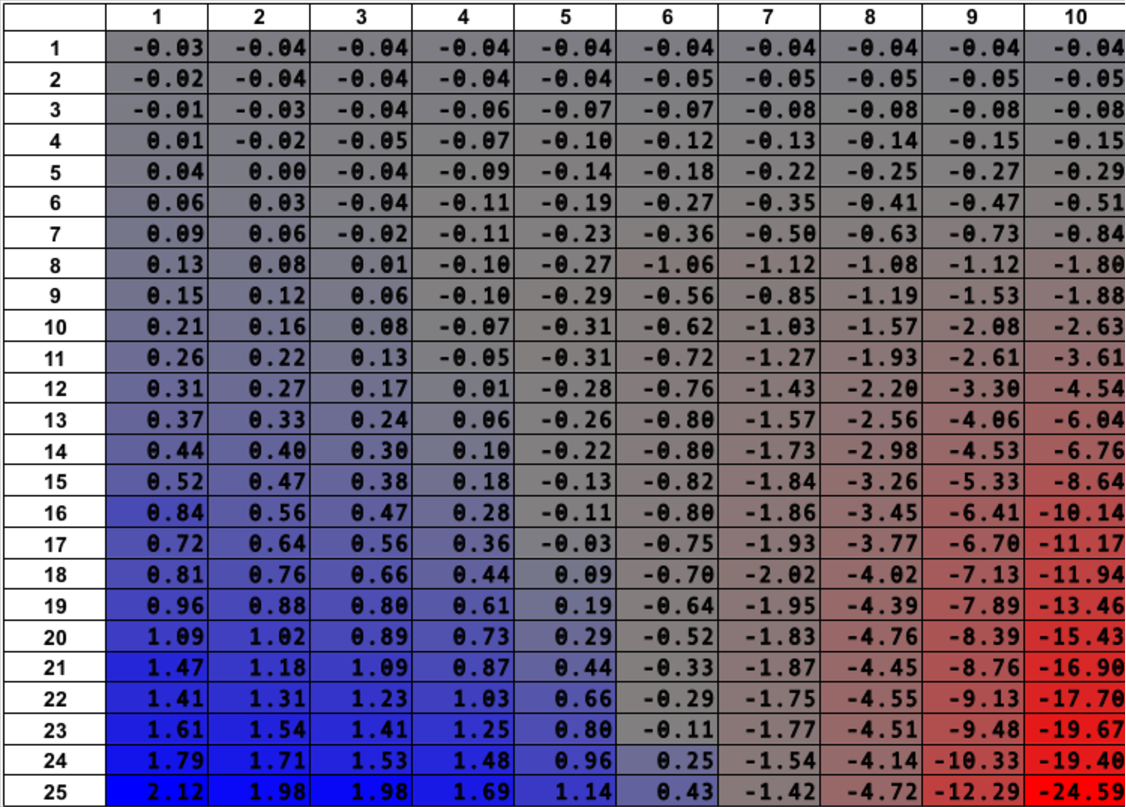
\includegraphics[
    page=1,
    width=\textwidth,
    height=\textheight,
    keepaspectratio
]{report_colors_cropped.pdf}
\vfill
\newpage

For formulas given in DNF, $cnf\_tt$ is faster for formulas of any length 
        sentences, and $cnf$ reaches Python's default maximum recursion depth 
        of $1000$ beginning at $3$ propositions.

The run time of $cnf$ is agnostic to the number of unique propositions
        in the given formula since uniqueness of a proposition is primarily
        semantic notion.
The semantic algorithm, $cnf\_tt$, is less concerned with the syntactic
        structure of the given formula since this has less bearing on the
        construction of a truth table.
The relative strengths of the two algorithms highlights two distinct ways that
        a propositional formula can be complex.
\end{document}
